\section{Structural context of low-scoring panel alleles (RCSB PDB, negative)}
A natural reason for AlphaMissense to miss damaging alleles is that it models
a single chain, so damage at a partner interface might be under-weighted. We
stated this as a falsifiable hypothesis --- alleles below the likely-pathogenic
threshold are \emph{enriched} at partner or ligand contact residues --- and
tested it on four experimental complexes from the RCSB PDB
(Table~\ref{tab:structure}). For each residue we computed relative solvent
accessibility (RSA) of the isolated chain with the Biopython Shrake--Rupley
implementation (maximum ASA from Tien et al.\ 2013) and contact with any
partner chain, DNA, or bound ligand (any heavy atom within 5\,\AA, Biopython
NeighborSearch). Author numbering was checked residue by residue against the
UniProt canonical sequence, and an allele was mapped only when its reference
amino acid matched the structure: 471 of 537 panel missense alleles mapped
(\texttt{results/structure\_panel\_alleles.csv}).

\begin{table}[h]\centering\footnotesize
\caption{Structures used. Identity = share of modelled residues matching UniProt.}\label{tab:structure}
\begin{tabular}{p{1.4cm}p{1.6cm}p{1.2cm}p{1.4cm}p{1.4cm}p{1.4cm}p{1.4cm}}
\hline
Gene & PDB (chain) & residues & identity \% & partner contacts & ligand contacts & alleles mapped \\ \hline
KRAS & 6VJJ (A) & 168 & 96.4 & 24 & 32 & 29 \\
TP53 & 1TSR (B) & 194 & 100.0 & 20 & 6 & 285 \\
CDKN2A & 1BI7 (B) & 125 & 99.2 & 35 & 0 & 70 \\
SMAD4 & 1U7F (B) & 193 & 100.0 & 65 & 0 & 87 \\
\hline\end{tabular}\end{table}

\paragraph{Control.} Buried residues score higher, as they should:
Spearman $\rho$(RSA, AlphaMissense) $=-0.114$ ($p=0.013$); REVEL $\rho=-0.100$
($p=0.029$); CADD, which has no structural input, shows none ($\rho=0.012$,
$p=0.8$).

\paragraph{Result: the hypothesis is falsified in the opposite direction.}
Low-scoring alleles are \emph{depleted} at contact residues: 3/27 versus 160/444
for the rest (Fisher OR 0.22, $p=0.0066$; protein/DNA partner contacts alone 2/27
versus 114/444, $p=0.036$). They are also less often buried (15/27 versus 352/444, OR
0.33, $p=0.0074$). Both effects hold jointly with gene fixed effects in a logistic
model (RSA coefficient 6.20, $p=6.4\times10^{-5}$; contact coefficient -2.18, $p=0.0022$).
\textbf{Verdict:} AlphaMissense's low scores fall mostly on exposed,
non-contact residues, where low damage is structurally plausible;
interface blindness does not explain them. The main exception is CDKN2A H83Y,
which is fully buried (RSA 0.00) in the p16 ankyrin fold yet scored benign.
The CDK6--p16 structure is 3.4\,\AA, and the p53 interface here is DNA only
(other p53 partners are not modelled), so contact calls are a lower bound.

\begin{figure}[h]\centering
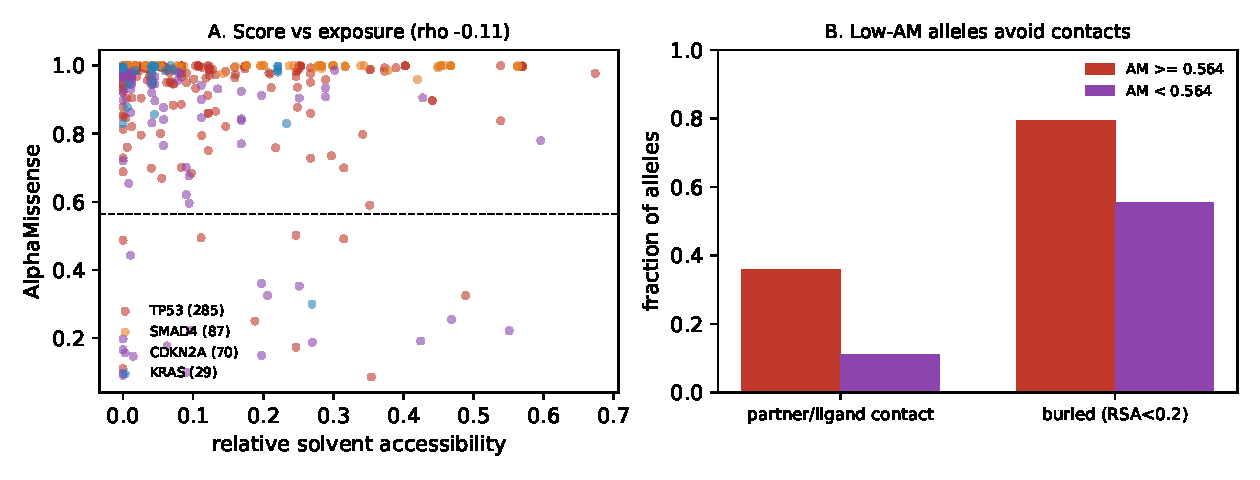
\includegraphics[width=0.85\linewidth]{figs/fig_structure.pdf}
\caption{A: AlphaMissense versus relative solvent accessibility for mapped
panel alleles. B: low-scoring alleles are less often at partner/ligand
contacts and less often buried.}\label{fig:structure}\end{figure}
